\section{Architecture}\label{sec:arch}

Our choice for the implementation of \cordic{} algorithm for Cartesian to polar
coordinates transformation is a \standout{pipelined architecture}. This choice
has been driven from the typical features that pipelines can achieve. High clock
frequency and, as direct consequence, an high throughput. This architecture is
particularly suitable in systems that need to process continuous streams of
data, in fact the pipeline need some clock cycles to be filled and to be
flushed.

\subsection{Block diagram}

\figref{fig:blockdiagram} shows the block diagram of our implementation. It
consists of three modules:
\begin{enumerate*}[label=]
	\item a container, that contains the other modules;
	\item a pre-rotation module;
	\item multiple stages connected in pipeline.
\end{enumerate*}

\begin{figure}[p]
	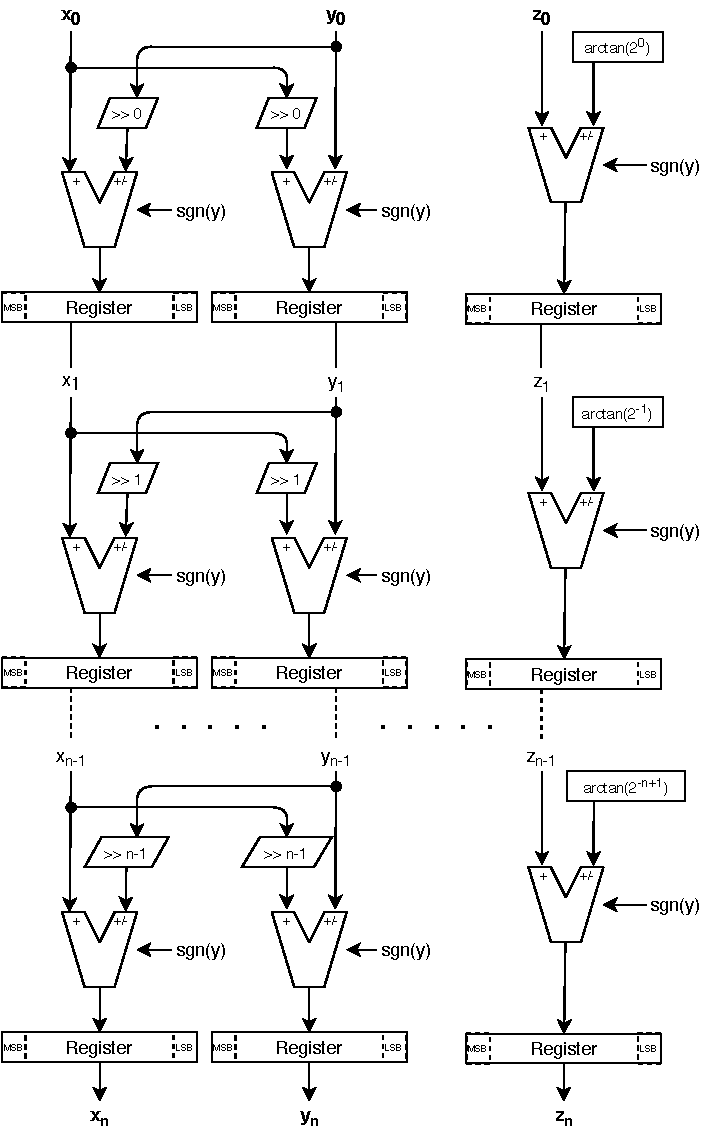
\includegraphics[width=\textwidth]{pipeline}
	\caption{Block diagram of the chosen architecture (pipelined).}\label{fig:blockdiagram}
\end{figure}

\subsubsection{Container Module}

The container module has as input two 16-bit words (x and y coordinates), the
clock and the reset. The inputs are supposed to be the quantization of
normalized real world values in the range \(\interval{-1}{1}\).

The outputs are two 20-bit words, the phase and the module.

Inside the container module we have two distinct types of submodule, a
pre-rotation module, and many pipeline stages.

\subsubsection{Pre-rotation Module}

This module has as input the x and y values on 16 bits and as output the
extended and rotated values and the initial phase offset, which can be \(0\),
\(\pi\) or \(-\pi\). This module will perform preprocessing needed to make the
algorithm converge. As we know the \cordic{} algorithm convergence is guaranteed
if the inputs are in the 1\textsuperscript{st} or the 4\textsuperscript{th}
quadrant of the Cartesian plane. This is because the values for the rotations
performed by the algorithm are fixed and the sum of this angles converges.
% FIXME: the sum of this angles converges (?!?)

The output is extended on 20 bits because we have to take in account the bit
growth in the pipeline that will be of \(\left\lceil{\log_2(n)}\right\rceil\),
where \(n\) is the number of iterations.

The initial phase offset has been dimensioned on 20 bits too for the same
reasons of \(x\) and \(y\). Note that in this case we don't have a real input on
16 bits for the phase, but we have done the quantization of the phase using 16
bits, so that the bit growth can be handled in the same way of \(x\) and \(y\).

The choice of the number of iterations has been done looking at the result of
the quantization of the angles. Values smaller then \(2^{-13}\) are quantized to
zero, thus steps after the 14\textsuperscript{th} will not have any influence on
the output phase.

\subsubsection{Pipeline Stages}

The other submodule type we can find inside the main container module is the
Pipeline Stage. This submodule performs the core of the \cordic{} algorithm, it
has as input three 20-bit words \(x_i\), \(y_i\), and \(phase_i\) and as output
again three 20-bit words \(x_{(i+1)}\), \(y_{(i+1)}\) and \(phase_{(i+1)}\). The
output of each stage will be the input of the next one, the first stage will
take as input the output of the pre-rotation module, the last one's output will
be used as output of the main module, using \(x_{last}\) as radius and
\(phase_{last}\) as phase, while \(y_{last}\) is not used.
